\documentclass[10pt,conference,compsocconf]{IEEEtran}

\usepackage{hyperref}
\usepackage{graphicx}
\usepackage{booktabs}
\usepackage{amsmath}
\usepackage{amssymb}

\begin{document}
\title{Predicting self-reported heart disease\\ in the 2015 BRFSS}

\author{CS-433 Project 1}

\maketitle

\begin{abstract}
We predict whether an adult in the 2015 Behavioral Risk Factor Surveillance System
has been told they had a heart attack or coronary heart disease.
Of 328{,}135 labelled rows, 8.83\% are positive, so a constant negative rule already
reaches accuracy 0.912 and F1 of 0.
The leaderboard metric is class-1 F1.
We focus on how the raw survey is turned into a design matrix.
Survey machinery and label leaks are removed; remaining codes are treated as
categories; the 300 one-hot levels with the largest mutual information with the
label are kept.
On that matrix, several linear models give similar F1.
Changing the preprocessing changes F1 by much more.
A neural net and a gradient-boosted tree are still to be evaluated; this draft
leaves their results open.
The current submission file is \texttt{submissions/weighted\_logistic.csv}.
\end{abstract}

\section{Problem and data}
The label is the BRFSS derived item for myocardial infarction, angina, or coronary
heart disease, stored as $\{-1,+1\}$.
The hidden test file has 109{,}379 rows and the same 321 columns.
We report class-1 F1 as the selection metric and precision-recall AUC beside it,
because PR-AUC does not depend on the decision cutoff.

The positive rate is not uniform across people.
It is about 1\% under age 45 and much higher for older men.
One score and one cutoff have to cover both groups.
Train and held-out F1 on linear models differ by about 0.01, so the limit looks
like class overlap rather than a solver that overfits a particular fold.

\section{Preprocessing}
Most of the work in this project is here.
Columns that describe how the interview was run (state, dates, phone checks,
sampling weights) are dropped first.
Four items that are answered only after a cardiac event, or that start because
of one (\texttt{HAREHAB1}, \texttt{STREHAB1}, \texttt{CVDASPRN}, \texttt{ASPUNSAF}),
are removed so the model cannot see the outcome.

Raw BRFSS codes are not magnitudes.
On day counts, 88 means zero days and 77 or 99 mean refused or unknown.
Treating those integers as real values pulls the feature in the wrong direction.
We therefore encode each kept column as levels:
a value held by at least 1\% of the fit rows becomes its own indicator;
rarer values are cut into at most five quantile bins;
missing is its own level when it is common enough.
Constant and duplicate level columns are discarded.
Mutual information with the label then keeps the top 300 levels, which are
standardized.
Levels, the ranking, and the scales are fit on training rows only and frozen
for validation and test.

\subsection{What else we tried}
With the same linear model, other designs scored lower.
Reading codes as numbers with a median fill and missing flags loses about
0.017 F1 relative to the one-hot path above.
Missing flags alone keep only the blank pattern and lose about 0.08 F1.
A hand codebook that maps each item to a clinical yes/no or ordered code, then
fills the mode and adds age and body-mass products, lands near 0.422 F1.
Keeping every one-hot level (about 1{,}750 columns) or adding age-interaction
products of those levels does not beat selecting 300 levels by mutual information.
The message is consistent: the representation of the survey moves the score;
small changes to a linear head do not.

\section{Models}
Let $y_i\in\{0,1\}$ and let $x_i\in\mathbb{R}^{d}$ be a standardized row after
preprocessing.
Logistic regression models
\begin{equation}
  p(y_i=1\mid x_i)
  =
  \sigma(\theta_0 + x_i^{\top}\theta_{1:})
  ,
  \qquad
  \sigma(z)=\frac{1}{1+e^{-z}}.
\end{equation}
With row weights $w_i$ (positives together weigh twice the negatives) and an
$\ell_2$ penalty on the non-bias weights, the training problem is
\begin{equation}
\label{eq:obj}
\min_{\theta}\;
\frac{1}{n}\sum_{i=1}^{n}
w_i\,\ell\!\left(y_i,\theta_0+x_i^{\top}\theta_{1:}\right)
+\lambda\|\theta_{1:}\|_2^2 ,
\end{equation}
where $\ell(y,s)=-y s+\log(1+e^{s})$ is the logistic negative log-likelihood
and $\lambda=10^{-5}$.
The bias is not penalized.
We minimize~\eqref{eq:obj} with 300 steps of accelerated proximal gradient (FISTA).
A row is predicted $+1$ when its score is at least a cutoff $t$.
Inside each outer training fold, 15\% of the rows (stratified) choose the $t$
that maximizes class-1 F1; the outer fold is scored once.
There are five folds, seed 42.
For the submission file the same 85/15 split is applied to every labelled row;
the test matrix is used only at prediction time.

\subsection{Linear comparisons}
On one prepared validation split we also fit the course full-batch logistic
regression, a mini-batch SGD logistic, and ridge regression.
Their F1 values sit in a narrow band.
Earlier runs of the six course solvers on a related design landed between about
0.42 and 0.43 validation F1.
That is the sense in which ``the model does not change the story'': once the
matrix is fixed, swapping among these linear methods moves F1 by a few
thousandths, while swapping the matrix (numeric codes versus one-hot levels,
flags only versus answers) moves it by one or more hundredths.

\subsection{Nonlinear models (pending)}
A linear score can change a feature's effect only through product columns that
were written by hand.
A gradient-boosted tree and a small neural net can learn such interactions from
data.
We plan to train both on the same outer folds and the same F1 cutoff protocol,
so their numbers are comparable to Table~\ref{tab:results}.
Those rows are left blank until the runs finish.

\section{Results}
Table~\ref{tab:results} summarizes what is ready.
The one-hot mutual-information matrix with weighted logistic regression is the
current submission; it is not claimed as a final winner over the pending models.

\begin{table}[t]
\centering
\caption{Five-fold means where available. Empty cells: not run yet.}
\label{tab:results}
\scriptsize
\begin{tabular}{lcccc}
\toprule
Setup & F1 & PR-AUC & ROC & cols \\
\midrule
One-hot MI top 300 + weighted logistic
  & 0.427 & 0.388 & 0.861 & 300 \\
Course logistic GD (same matrix, one split)
  & --- & --- & --- & 300 \\
SGD logistic (same matrix, one split)
  & --- & --- & --- & 300 \\
Ridge (same matrix, one split)
  & --- & --- & --- & 300 \\
Gradient boosting (planned)
  & --- & --- & --- & --- \\
Neural net (planned)
  & --- & --- & --- & --- \\
\midrule
\multicolumn{5}{l}{\emph{Earlier preprocessing checks (same linear family)}} \\
Codebook recode + mode fill
  & 0.422 & 0.386 & 0.859 & 171 \\
Median fill + missing flags
  & 0.410 & 0.359 & 0.851 & 464 \\
Missing flags only
  & 0.343 & 0.270 & 0.807 & 187 \\
\bottomrule
\end{tabular}
\end{table}

Figure~\ref{fig:cm} pools the five test folds of the current submission.
Pooled precision is about 0.355, recall about 0.537, F1 about 0.427.
Most errors are false alarms: of about 29{,}000 positive rows, roughly half are
missed and a larger number of negatives are called positive.

\begin{figure}[t]
\centering
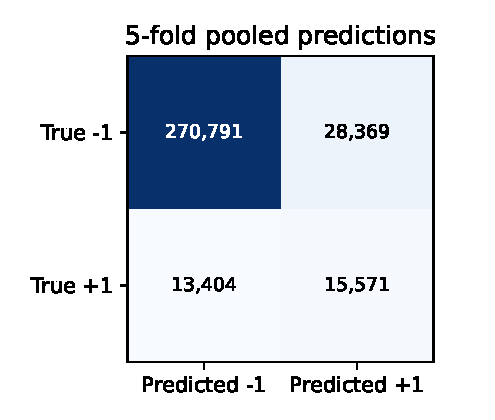
\includegraphics[width=0.92\columnwidth]{confusion_weighted_logistic.pdf}
\caption{Pooled predictions of the current linear submission. Each cell is a count over the five test folds.}
\label{fig:cm}
\end{figure}

Permutation importance on a one-hot fold points to sex, prior stroke, general
health, and cholesterol-related items among the largest drops in PR-AUC.
Age is split across many level columns, so a single raw age name looks weaker
even though age levels remain in the matrix.

\section{Conclusion}
Preprocessing is the lever that moved F1 in this project.
Treating survey codes as categories and selecting levels by mutual information
beats reading the same codes as numbers or keeping only missingness.
Among linear models on a fixed matrix, the differences are small.
We therefore submit a simple weighted logistic regression on the selected
one-hot design, and we leave space in the results for a gradient-boosted tree
and a neural net under the same evaluation protocol.
The public score of the submission file is still unknown and should be compared
with the five-fold estimate rather than with the cutoff-selection slice alone.

\end{document}
